En este capítulo se observan las diferentes pantallas que responden a las consultas realizadas a la MIB desde Linux y desde Windows.
\section{Cuestionario}
\begin{enumerate}
\item ¿Cuándo fue el último reinicio (Dia, hora y minuto)  de los agentes?
\\ El resultado del último reinicio en Linux como se observa en la figura \ref{image:reinicio} fue:

\FloatBarrier
\begin{figure}[htbp!]
		\centering
			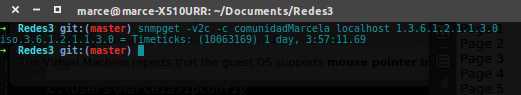
\includegraphics[width=.9 \textwidth]{images/Pregunta1}
		\caption{Último reinicio del agente en Linux.}
		\label{image:reinicio}
\end{figure}
\FloatBarrier

\item ¿Cuántas interfaces Ethernet tienen?
\\ Se puede observar en la figura \ref{image:interfaces} resultado en Linux fue de 0 interfaces Ethernet.
\FloatBarrier
\begin{figure}[htbp!]
		\centering
			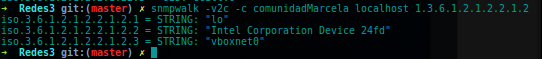
\includegraphics[width=.9 \textwidth]{images/Pregunta2L}
		\caption{Número de interfaces Ethernet en Linux.}
		\label{image:interfaces}
\end{figure}
\FloatBarrier

\item ¿Cuál es la velocidad (en MBPS) de esas interfaces?
\\ El resultado en Linux mostrado en la figura \ref{image:velocidadInterfaces} fue:
\begin{itemize}
\item lo = 100000000
\item Intel Corporation Device 24fd = 0 
\item vboxnet0 = 100000000
\end{itemize}
\FloatBarrier
\begin{figure}[htbp!]
		\centering
			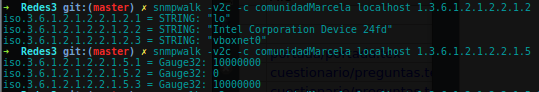
\includegraphics[width=.9 \textwidth]{images/Pregunta3L}
		\caption{Velocidad de las interfaces en Linux.}
		\label{image:velocidadInterfaces}
\end{figure}
\FloatBarrier

\item ¿Cuál es la interfaz que ha recibido el mayor número de octetos?
\item Indica el número de octetos  de la interfaz que ha recibido el mayor número de octetos
\item ¿Cuál es la MAC de esa interfaz?
\item ¿Cuál es la ip de la Interfaz que ha recibido el mayor número de octetos?
\item ¿Cuántos mensajes ICMP ha recibido el agente?
\item ¿Cuántas entradas tiene la tabla de enrutamiento IP?
\item ¿Cuántos datagramas UDP ha recibido el agente?
\item ¿El agente ha recibido mensajes TCP? ¿Cuántos?
\item ¿Cuántos mensajes EGP ha recibido el agente?
\item Indica el Sistema Operativo que maneja el agente.
\item Modifica el estatus administrativo (a down) de la interfaz que ha recibido más octetos.
\item Genera una alerta para avisar cuando se reinicie el agente.
\item Dibuja la MIB del agente.
\end{enumerate}